\chapter{A Highland Teosinte Introgression Modulates Phosphatidylcholine Levels and is Associated with Maize Flowering Time}
\label{chap-two}

\newrefsection

\section{Disclaimer}

\section{Abstract}

%%%%%%%%%%%%%%%%%%%%%%%%%%%%%%%%%%%%%%%%%%%%%%%%%%%%%%%%%%%%%%%%%%%%%%%5%
\section{Background}
%%%%%%%%%%%%%%%%%%%%%%%%%%%%%%%%%%%%%%%%%%%%%%%%%%%%%%%%%%%%%%%%%%%%%%%5%

%How do organisms adapt to high elevations
Elevation gradients are associated with changes in environmental factors that impose substantial physiological constraints on an organism. 
Adaptation to highland environments is achieved via the selection of genetic variants that improve their ability to withstand lower oxygen availability \citep{yi2010-se, bigham2010-is}, increased ultraviolet (UV) radiation \citep{yang2017-gs} and lower temperatures \citep{cicconardi2020-gs}.
In particular, cold temperatures reduce thermal time accumulation, measured in growing degree days (GDDs), \citep{gilmore1958-dx} and select for accelerated development and maturity as a compensatory mechanism \citep{hatfield2015-od}.
%Maize domestication and expansion
Following domestication from teosinte \parv (\textit{Zea mays} ssp. \parv) \citep{matsuoka2002-bg} in the lowland, subtropical environment of the Balsas River basin (Guerrero, M\'exico), cultivated maize (\textit{Zea mays} ssp. \textit{mays}) expanded throughout M\'exico and reached the highland valleys of central M\'exico around 6,500 years ago \citep{piperno2001-ea}.

%Contribution of mexicana to highland maize adaptation.
In M\'exico, highland adaptation of maize was aided by substantial adaptive introgression from a second teosinte subspecies, teosinte \mex (\textit{Zea mays} ssp. \mex), that had already adapted to the highlands of M\'exico thousands of years after its divergence from teosinte \parv \citep{hufford2013-gs, gonzalez-segovia2019-jy}. 
Adaptation to low temperature and soils with low phosphorus content in highland environments drove \mex genetic divergence from the lowland \parv \citep{aguirreliguori2019-fl}.
Phenotypically, the most evident signs of \mex introgression into maize are the high levels of stem pigmentation and pubescence \citep{lauter2004-eq} that are thought to protect against high UV radiation and low temperatures. 
The ability to withstand low temperatures and efficiently photosynthesize during the early stages of seedling development are key factors in maize highland adaptation \citep{hardacre1980-tq}.
Indeed, recent transcriptome deep sequencing (RNA-seq) analysis showed that the inversion \textit{Inv4m}, introgressed from \mex, strongly affects the expression of genes involved in chloroplast physiology and photosynthesis \citep{crow2020}.  
Given the slow accumulation of GDDs in typical highland environments, selection has favored shorter generation  times in highland adapted maize \citep{gates2019-xu}.
By the time maize reached the Mexican highlands, its range had already expanded far to the South, including the colonization of highland environments in the  Andes \citep{athens2016-ep, grobman2012-pm}. 
Andean maize adaptation occurred largely independently of \mex introgression \citep{takuno2015-uj, wang2020-mp}, and there is no known wild teosinte relative in South America. 
These multiple events of maize adaptation to highland environments make maize a good system to study the evolutionary and physiological mechanisms of convergent adaptation \citep{takuno2015-uj, wang2020-mp}.

%Photoperiod adaptation
In comparison to its southward expansion, the northward migration of maize into the modern-day United States, where summer daylengths are longer, occurred at a much slower pace \citep{da_fonseca2015-zh, swarts2017-ge} due to delayed flowering of photoperiod-sensitive tropical maize lines \citep{hung2012-ms}.
A host of evidence suggests that maize cultivation in northern latitudes was enabled by the selection of allelic variants that led to a reduction in photoperiod sensitivity to allow flowering under longer photoperiods \citep{liang2018-af, guo2018-on, coles2010-db, huang2018-ga, yang2013-lg, salvi2007-ku, hung2012-ms}.
Some of the early flowering alleles that conferred an adaptive advantage in highland environments are the result of \mex introgressions into highland maize \citep{guo2018-on}.
Maize first entered into the US via the Mexican highlands \citep{da_fonseca2015-zh}, and these early flowering alleles show further evidence of selection in northern latitudes \citep{guo2018-on}, consistent with a likely role for \mex introgression(s) in maize adaptation to shorter daylength. 
When introduced into Northern Europe, photoperiod-insensitive maize from the Northern US and Canada thrived as it was already pre-adapted to northern latitudes and lower temperatures \citep{brandenburg2017-ii}.
The genetic, physiological, and phenotypic basis of these adaptations, however, is quite limited.

Plant phospholipids, as well as other glycerolipids such as sulfolipids, galactolipids, and non-polar lipids such as triacylglycerols, are involved in plant responses to low temperatures.
Phospholipid levels are increased in plants exposed to low temperatures \citep{degenkolbe2012-wf} and levels of unsaturated fatty acids in glycerolipids are reduced \citep{welti2002-uk, lynch1987-ln}, which may help maintain the fluidity of cell membranes.
Under stressful conditions, the proportions of differently shaped lipids are modulated to maintain membrane flexibility while preventing membrane leakage. 
For instance, phosphatidylcholines (PCs) are rectangular polar lipids that are well suited for the formation of bilayer membranes because the size of their glycerol backbone, choline headgroup and fatty acid tails are similar.
By contrast, lyso-phosphatidylcholine (LPC) is a triangular PC with a single acyl group that cannot form a bilayer because its headgroup is much larger than its fatty acid \citep{jouhet2013-fv}.
LPCs do allow for some membrane movement, but high LPC concentrations act as a detergent \citep{henriksen2010-cm} and can facilitate cell leakage and damage at low temperatures, effects that would be prevented by higher PC levels.
In cold-adapted maize temperate lines and \textit{Tripsacum} species (a distant maize relative), genes involved in  phospholipid biosynthesis show accelerated rates of protein sequence evolution, further supporting an important role for phospholipid metabolism across several species during cold adaptation \citep{yan2019-tx}. 
Finally, multiple phospholipids can bind to Arabidopsis (\textit{Arabidopsis thaliana}) FLOWERING LOCUS T (FT) and accelerate flowering.
Recent work has shown that phosphatidylglycerol binds and sequesters FT in companion cells in low temperatures, while higher temperatures release it to the shoot apical meristem \citep{susila2021-dz}.
There, it interacts with certain species of PC, the most abundant phospholipid in plant cells \citep{gu2017-nd},  through an unknown mechanism \citep{nakamura2014-qf}. 
Consistent with this observation, glycerolipid levels in maize have predictive power for flowering time \citep{riedelsheimer2013-bd}. 

Here, I identified an adaptive teosinte \mex introgression that alters highland maize phospholipid metabolism and leads to early flowering.
Using genome scans and linkage mapping,  identified \textit{High PhosphatidylCholine1} (\hpc), a gene encoding a phospholipase A1, as a driver of high PC levels in highland maize. 
Data from thousands of genotyped landrace test-crosses grown in common garden experiments at different elevations in M\'exico showed a strong genotype-by-environment effect at the \hpc locus, where the highland allele leads to higher fitness in the highlands and reduced fitness at lower elevations.
Furthermore, we determined that the highland \hpc allele, which was introgressed from teosinte \mex, was carried northward and is now present in maize cultivars grown in the Northern US and European Flint lines.
These results suggest that the \hpc highland allele has a beneficial effect in cold, high-latitude environments, where early flowering is advantageous


%%%%%%%%%%%%%%%%%%%%%%%%%%%%%%%%%%%%%%%%%%%%%%%%%%%%%%%%%%%%%%%%%%%%%%%5%
\section{Methods}
%%%%%%%%%%%%%%%%%%%%%%%%%%%%%%%%%%%%%%%%%%%%%%%%%%%%%%%%%%%%%%%%%%%%%%%5%

\subsection{Plant Materials}
The diversity panels and mapping populations used in this manuscript for population genetics measures of selection, QTL mapping and G x E analysis have been described previously by \citep{wang2020-mp}, \citep{gates2019-xu}, \citep{romero_navarro2017-cn}, \citep{janzen2021-lz} and \citep{perez-limon2022-lg}. 

\subsection{Genome Scan for Local Adaptation}
In order to conduct genome scans for signatures of adaptation we used the \textit{pcadapt} \citep{luu2017-ws} package.
\textit{pcadapt} identifies adaptive loci by measuring how strongly loci are contributing to patterns of differentiation between major axes of genetic variation.
Under simple models \textit{pcadapt} captures major patterns of $F_{ST}$  but is conducted in a way that does not require population delimitation \citep{duforet2014genome}.
As the genome scan comparison requires a focal SNP to be compared to the first K principal components of the genotype data, it can be biased by large regions of low recombination that drive the major axes of variation in the principal components.
Thus, when SNPs from these low recombination regions are compared against principal components driven by linked loci spurious signals may arise.
To prevent this bias from occurring, we used custom scripts to calculate the principal component step separately based upon all the chromosomes except for the chromosome of the focal SNPs being tested.
The genotype data we used for this analysis was GBS data from roughly 2,000 landraces of Mexican origin collected by CIMMYT (www.cimmyt.org) as part of the SeeDs of discovery initiative (\href{https://www.cimmyt.org/projects/seeds-of-discovery-seed/}).
From this, we calculated the strength of association between each SNP and the first five principal components (excluding the chromosome of the focal SNP) using the communality statistic as implemented in \textit{pcadapt} version 3.0.4.


\subsection{Glycerolipid pathways selection}
We compiled a list of genes pertinent to glycerolipid metabolism starting with a search of all genes belonging to the \textit{Zea mays} 'Glycerophospholipid metabolism' and 'Glycerolipid metabolism' KEGG pathways \citep{kanehisa2019} (map identifiers: zma00564 and zma00561). 
With the NCBI Entrez gene identifiers in KEGG we retrieved the AGPv4 transcript identifiers used in Corncyc 8.0 \citep{portwood2019, walsh2016} from an id cross reference \href{https://www.maizegdb.org/search/gene/download_gene_xrefs.php?relative=v4}{file} found in MaizeGDB   \citep{portwood2019}.
This resulted in a list of 300 genes comprising 51 Corncyc pathways. 
Then we discarded Corncyc pathways  tangentially connected to the KEGG glycerolipid metabolism list (sharing just one enzyme with the initial KEGG list) or that we judged to belong to different biological processes (e.g 'long chain fatty acid synthesis','anthocyanin biosynthesis'). 
Finally, we added manually the 'phosphatidylcholine biosynthesis V' pathway that was missing. 
The list of 30 selected Corncyc pathways included genes outside the initial KEGG search results and raised the number of genes to 557. 
In addition to these, 37 genes were found to have an enzymatic activity related to phospholipid metabolism but not placed into any particular pathway, i.e orphan enzymes, consisting mostly of alcohol dehydrogenases. 
Sixteen additional genes found in KEGG were not annotated at all in Corncyc probably due to differences between AGPv4 and RefSeq pseudogene annotation of the maize genome. 
The list of all possible candidates coming either from KEGG or Corncyc that were orphan enzymes or were unannotated in Corncyc amounted to 597 genes (Sup. File 2). 
This process is documented in the \verb|0_get_glycerolipid_genes.R| script of the \verb|pgplipid| R package accompanying this paper \citep{fausto_rodriguez_zapata_2020_4323410}.

\subsection{Population Branch Excess Analysis}
Population Branch Excess quantifies changes in allele frequencies in focal populations relative to two independent “outgroup” populations.
We used \textit{Zea mays spp. parviglumis} as one of the outgroup populations for all four highland groups.  
The other outgroup was  Mexican lowlands  in the case of Southwestern US , Mexican highlands and Guatemalan highlands; and South American lowlands in the case of the Andes population. 
We used calculated PBE SNP values for the four populations (described in detail in \citep{wang2020-mp}) and we tested for selection outliers SNPs in the 594 phosphoglycerolipid-related candidate genes and the 30 Corncyc pathways (556 genes).
We first defined PBE outlier SNPs as the top 5\% of the PBE score distribution; this fraction corresponds to approximately 50000 out of ~1 million genotyped SNPs in each population. 
Following \citep{wang2020-mp}, we defined a gene as a PBE outlier if it contained an outlier SNP within the coding sequence or 10 kb upstream/downstream. 
Then we tested for over-representation of genes selected in particular subsets of populations using Fisher's exact test with the 32,283 protein-coding genes from the maize genome as background. 
For each pathway, we first selected all SNPs within coding regions and 10 kb upstream and downstream of genes in the pathway and we calculated the mean pathway PBE score. 
We then constructed a null distribution by drawing 10,000 samples without replacement of $n$ SNPs from those found within 10 kb upstream and downstream of all protein-coding genes and we obtained the mean PBE for this null distribution. 
With the set of PBE outliers for glycerolipid metabolism in the four populations, we tested for evidence of physiological or pleiotropic constraint using the $C_\chi^2$ statistic \citep{yeaman2018}. 

\subsection{QTL analysis of phospholipid levels}
We analyzed glycerophospholipid QTLs in a mapping population of 57 RILs (BC1S5) from the cross B73 x PT.
These RILs were grown in a highland site in Metepec, Edo de M\'exico at 2,600 masl during the summer of 2016 and in Puerto Vallarta, Jalisco at 50 masl during the winter of 2016/17. 
We analyzed the samples using UHPLC-QTOF, as above, and 67 leaf lipid species were identified.
For QTL analysis we calculated the mean across all fields of individual lipid mass signal. 
We also used as phenotypes the sum total of the following lipid classes: diacylglycerols, triacylglycerols, PCs and  LPCs.  
Furthermore,  we also included the log base 10 transformed ratios of LPCs/PCs and the ratios of their individual species. 
We did a simple single marker analysis  with ``scanone`` using Haley-Knott  regression, and assessed the QTL significance with 1,000 permutations.

\subsection{CRISPR-Cas9 editing of \hpc and analysis of the effect of \textit{hpc1\textsuperscript{CR}} mutant on flowering time}
CRISPR/Cas9 was used to create a \hpc mutant through Agrobacterium \textit{Agrobacterium tumefaciens}-mediated transformation of background line B104 \citep{Wu2020-nq, Char2017-uk}. 
RNA guides (gRNAs) were designed as described in \citep{Brazelton2015-co} for the B73 reference genome v4. 
The B104 and B73 sequence for \hpc were identical. 
The gRNA cassette was cloned into pGW-Cas9 using Gateway cloning. 
Two plants from the T\textsubscript{0} transgenic events were identified through genomic PCR amplification and Sanger sequencing and were self-pollinated. 
In the next generation, several plants were allowed to self.
Plants were genotyped using forward primer CAGTTCTCATCCCATGCACG and reverse primer CCTGATGAGAGCTGAGGTCC.


\subsection{Haplotype network analysis of \hpc in Mexican maize landraces and teosintes}
We extracted SNP genotypes for \hpc from the TIL teosinte accessions in the HapMap 3 imputed data \citep{bukowski2017-ng} and the 3700 Mexican landraces in the SeeD dataset. 
With the set of 1060 accessions that were homozygous at all sites in this genomic region we calculated a haplotype network depicting the minimal spanning tree for haplotypes covering 90\% of the input accessions with the R package \code{pegas} \citep{paradis2010}, and haplotype frequencies for three elevation classes in the landraces (0--1,000; 1,000--2,000 and >3,000 masl).
\subsection{Clustering analysis of \hpc in maize inbred lines and teosintes}
Using v3 of the B73 genome, \hpc SNPs were obtained from PT (this paper), the 282 diversity panel \citep{flint-Garcia2005-hb}, teosinte inbred lines and the German inbred lines from HapMap 3 \citep{bukowski2017-ng}. 
The selection was made to have a good representation of tropical, temperate and European inbred lines together with teosintes and PT lines.
SNPs were aligned using Geneious2020.0.5 and a neighbor-joining cluster analysis was generated. 
To facilitate visualization and interpretation of the tree we condensed cluster branches from lines with identical haplotypes and from similar geographic locations. 
The full tree is available as Sup. file 9. 
\subsection{Expression analysis of candidate genes and association with flowering traits in the 282 diversity panel}
We used gene expression RNA-seq data obtained from the 282 diversity panel at different developmental stages \citep{kremling2018-gn} and BLUP values of several flowering and photoperiod sensitivity traits \citep{hung2012-ms} to study the correlation of \hpc expression values with flowering time traits.  

\clearpage

\section{Results}

%%%%%%%%%%%%%%%%%%%%%%%%%%%%%%%%%%%%%%%%%%%%%%%%%%%%%%%%%%%%%%%%%%%%%%%%%%%%%%%%%%%%%%%
\subsection{Genes involved in PC/LPC conversion show strong highland selection signals} 
%%%%%%%%%%%%%%%%%%%%%%%%%%%%%%%%%%%%%%%%%%%%%%%%%%%%%%%%%%%%%%%%%%%%%%%%%%%%%%%%%%%%%%%
We selected a set of 597 maize glycerolipid genes from their functional annotations (see Materials and Methods) to identify selection signals using the Population Branch Excess (PBE) \citep{pool2017-oa} statistic across four highland populations: Southwestern US (SWUS), Mexican highlands (MH), Guatemalan highlands (GH) and Andes (AN) (\cref{Fig1}E) \citep{wang2020-mp}. 
We identified a significant excess of genes that are targets of selection in more than two populations ($ p< 3 \times 10^{-5}$, \ref{Fig1}F).
The most over-represented intersection of selected glycerolipid genes was between the SWUS, MH and GH populations ($p = 1  \times 10 ^{-15} $, \cref{Fig1}F), suggesting that genes were specifically selected in these three populations relative to the AN population and/or that there was closer kinship among SWUS, MH, and GH populations than the AN population and thus weaker statistical independence.
From all annotated glycerolipid genes, 23 were consistently PBE outliers across all four highland populations ($p =<1  \times  ^{-10}$, \cref{Fig1}F).
We then assigned a PBE value to each of the 30 glycerolipid metabolism pathways (using a 10 kb window around each constituent gene)  and compared their average PBE value with a genome-wide random sampling distribution of PBE values within genic regions. 
From these, we established that 'phospholipid remodeling' and 'PC acyl editing' exhibit significantly higher PBE values in all four populations, indicating a possible role for phospholipid remodeling in maize highland adaptation
(\cref{Fig1}G). 


\begin{figure}[htp]
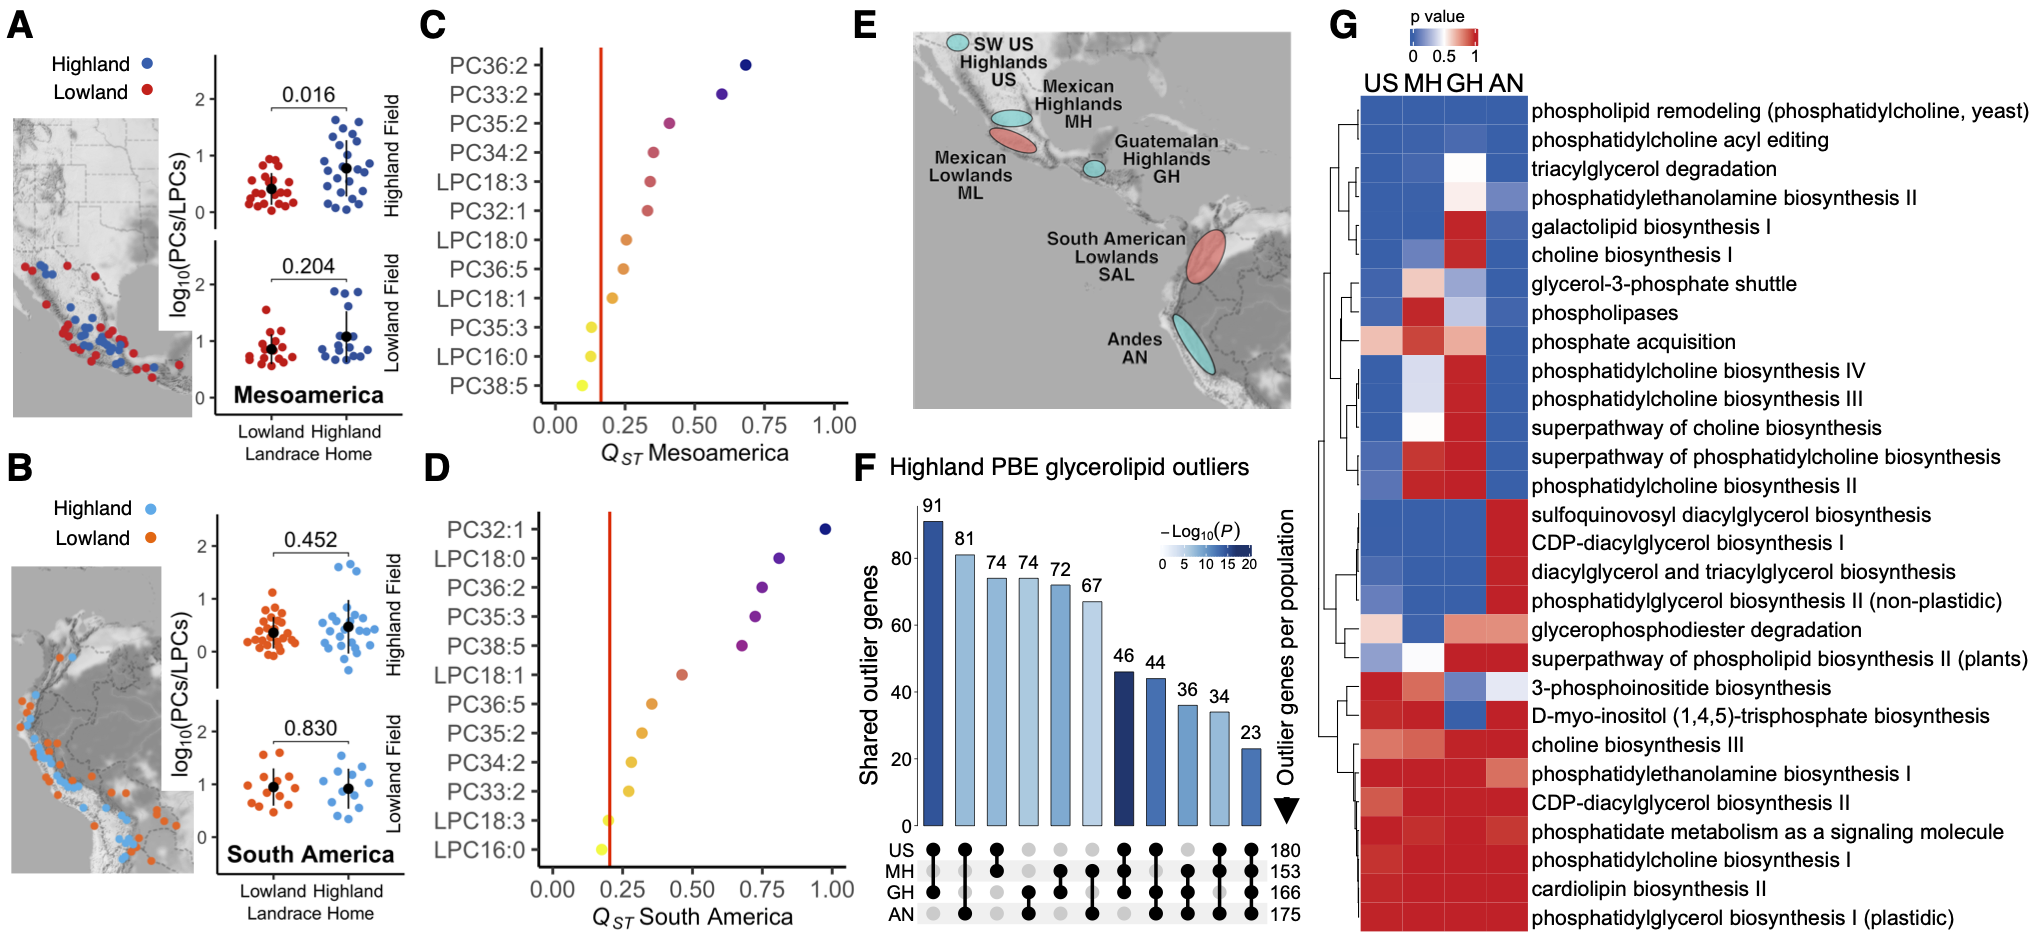
\includegraphics[width=\linewidth]{Chapter-1/figs/Fig_1.png}
\caption[Phospholipid selection in highland maize.]{\textbf{Phospholipid selection in highland maize.}} 
\textbf{(A-B)} \textit{Left:} Geographical origin of 120 maize accessions from the HiLo diversity panel used in the common garden experiment for glycerolipid quantitation.
\textit{Right:} PC/LPC ratio, log\textsubcript{10} scaled, for highland and lowland landraces from (A) Mesoamerica, $n=54$; and (B) South America, $n=53$. The black cirlce indicates the mean, the vertical line is the standard deviation (SD). Significant differences were tested with a false-discovery rate (FDR) adjusted \textit{t}-test; the resulting \textit{p}-values are shown.
\textbf{(C-D)}
\textit{$Q_{ST}$-$F_{ST}$} analysis of phospholipids between highland and lowland landraces from (C) Mesoamerica  and (D) South America. 
Red line, neutral $F_{ST}$ + 2 SD.
\textbf{(E-G)} Highland vs lowland Population Branch Excess (PBE) analysis.
\textbf{(E)} PBE geographical sampling.
\textbf{(F)} PBE outlier counts for glycerolipid genes in four highland populations.
Bar shade indicates Fisher's exact significance test for excess shared outliers. 
\textbf{(G)} Highland selection of glycerolipid-related pathways using PBE. The heatmap shows the probability of randomly sampling gene SNPs with mean PBE greater than the mean for the gene SNPs in each pathway.
\label{Fig1}
\end{figure}


\begin{figure}[ht]
\centering
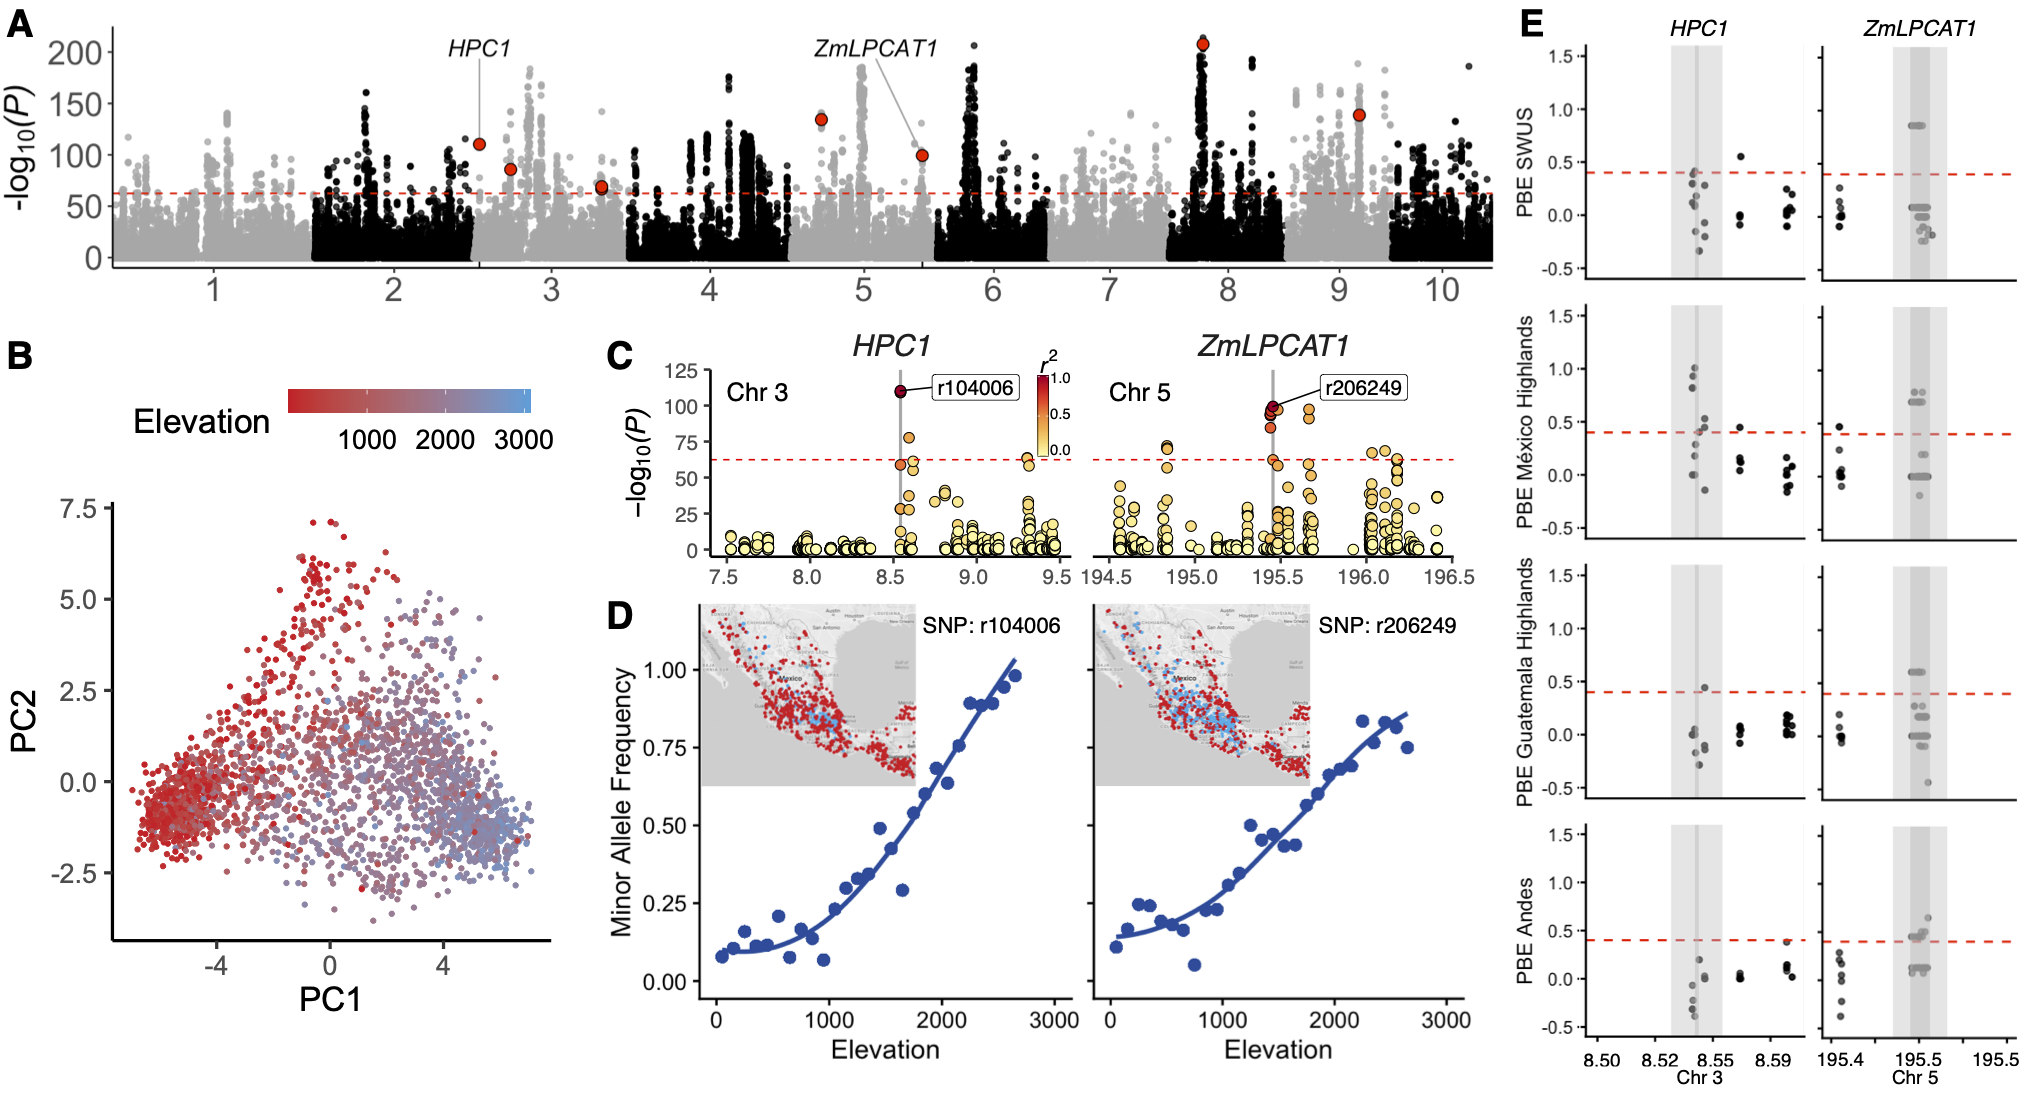
\includegraphics[width=\linewidth]{Chapter-1/figs/Fig_2.png}
\caption[Evidence of highland selection in genes determining PC/LPC ratios]{\textbf{\textit{Evidence of highland selection in genes determining PC/LPC ratios.}}
 \textbf{(A)} Association with genetic principal component 1 (PC1) from \textit{pcadapt} analysis of Mexican landraces (open pollinated varieties), dashed marks the top 5\% $-log_{10}(P)$. 
 Red points show SNPs in glycerolipid metabolism genes that are also PBE outliers for Mexican highlands (Supplementary Table 2). 
 From these, \hpc and \textit{ZmLPCAT1} are the top genes with orthologs catalyzing PC/LPC interconversion. 
 \textbf{(B)} Scatter plot of the \textit{pcadapt} first two genetic principal components illustrating that PC1 correlates with elevation.
 \textbf{(C)} Extended region from (A) of the 1 Mb interval around \hpc and \textit{ZmLPCAT1}. Linkage disequilibrium ($r^2$) with the peak SNP for each gene are illustrated by the color scale; both peak SNPs are located in the coding sequence. 
\textbf{(D)} Elevation clines for the peak SNPs from (C), the insets show the geographic distribution of the highland (blue) and lowland (red) alleles.
\textbf{(F)} Population Branch Excess of SNPs in \textit{ZmLPCAT1} and \hpc. Dark grey, coding sequence; light grey, 10 kb upstream and downstream; dashed line is the threshold for the top 5\% PBE value outliers.} 
\label{Fig2}
\end{figure}
\clearpage
We considered two possible explanations for the extent of convergent selection in highland populations (see explanations in \citep{wang2020-mp, yeaman2018}). 
Adaptation may be conferred by a small number of genes, thereby imposing a \textit{physiological} constraint on the sources of adaptation leading to convergence. 
Alternatively, adaptation may be the result of many genes, but deleterious \textit{pleiotropic} effects restrict the number of genes that can be targeted by selection, also leading to convergence.  
Using Yeaman's $C_{hyper}$ statistic \citep{yeaman2018}, which quantifies these two modes of convergent adaptation, we determined that the overlap among putative adaptive genes in the four highland populations cannot be explained merely by physiological constraints ($C_{hyper} = 3.96$, Supplementary Table 1). 
A certain degree of pleiotropic constraint is therefore likely.
Overlap between adaptation candidates was higher for the SWUS, MH and GH population pairs ($C_{hyper} = 4.79$) than between the Andean and SWUS, MH and GH pairs ($C_{hyper} = 3.14$).

To further understand selection at the gene level, we used genotyping by sequencing (GBS) data from 2,700 Mexican maize landraces, generated by the SeeD project \citep{romero_navarro2017-cn, gates2019-xu}, to run a \textit{pcadapt} \citep{luu2017-ws} analysis to determine how loci might contribute to observed patterns of differentiation along major principal components of genetic variation. 
The first \textit{pcadapt} principal component separated Mexican landraces based on the elevation of their geographical origin (\cref{Fig2}B).
Using this first principal component, we identified outlier single nucleotide polymorphisms (SNPs) across the genome that are significantly associated with genetic variation along elevation and potentially involved in local adaptation (\cref{Fig2}A).
From the list of $\approx 600$ maize glycerolipid-related genes, 85 contained SNPs that were \textit{pcadapt} outliers for association with the first genetic principal component (top 5\% $-log_{10}(P)$), and of which eight were also PBE outliers for Mexican highlands (\cref{Fig2}A, Supplementary table 2, Sup. File 2). 
These eight selection candidates, supported by two different sources of evidence, included two genes coding for putative enzymes whose orthologs are known to directly catalyze PC/LPC interconversion reactions. 
The first gene, Zm00001d039542, with a $-log_{10}(P)$ of $110.28$, encoded a putative phospholipase A1 that we name \textit{High PhosphatidylCholine 1}, \hpc.
The second gene, Zm00001d017584, with a $-log_{10}(P)$ of $99.31$, encoded a predicted \textit{Lyso-Phosphatidylcholine Acyl Transferase 1} that we will refer as \textit{ZmLPCAT1}. (\cref{Fig2}C). 
Although these two types of enzymes catalyze broadly opposite reactions (degradation vs biosynthesis of PC) they are unlikely to catalyze strictly reverse reactions in the Lands cycle. 
A1 phopholipases attack the phosphatidylcholine at the \textit{sn-1} carbon, while LPC acyl transferases usually acylate \textit{sn-2} \citep{wang2012,richmond2011}.
Instead, plant PLA1 enzymes like \hpc are better known for their role in the first step of jasmonic acid biosynthesis \citep{wang2018b, ishiguro2001-ob}.

\begin{figure}[!ht]
\centering
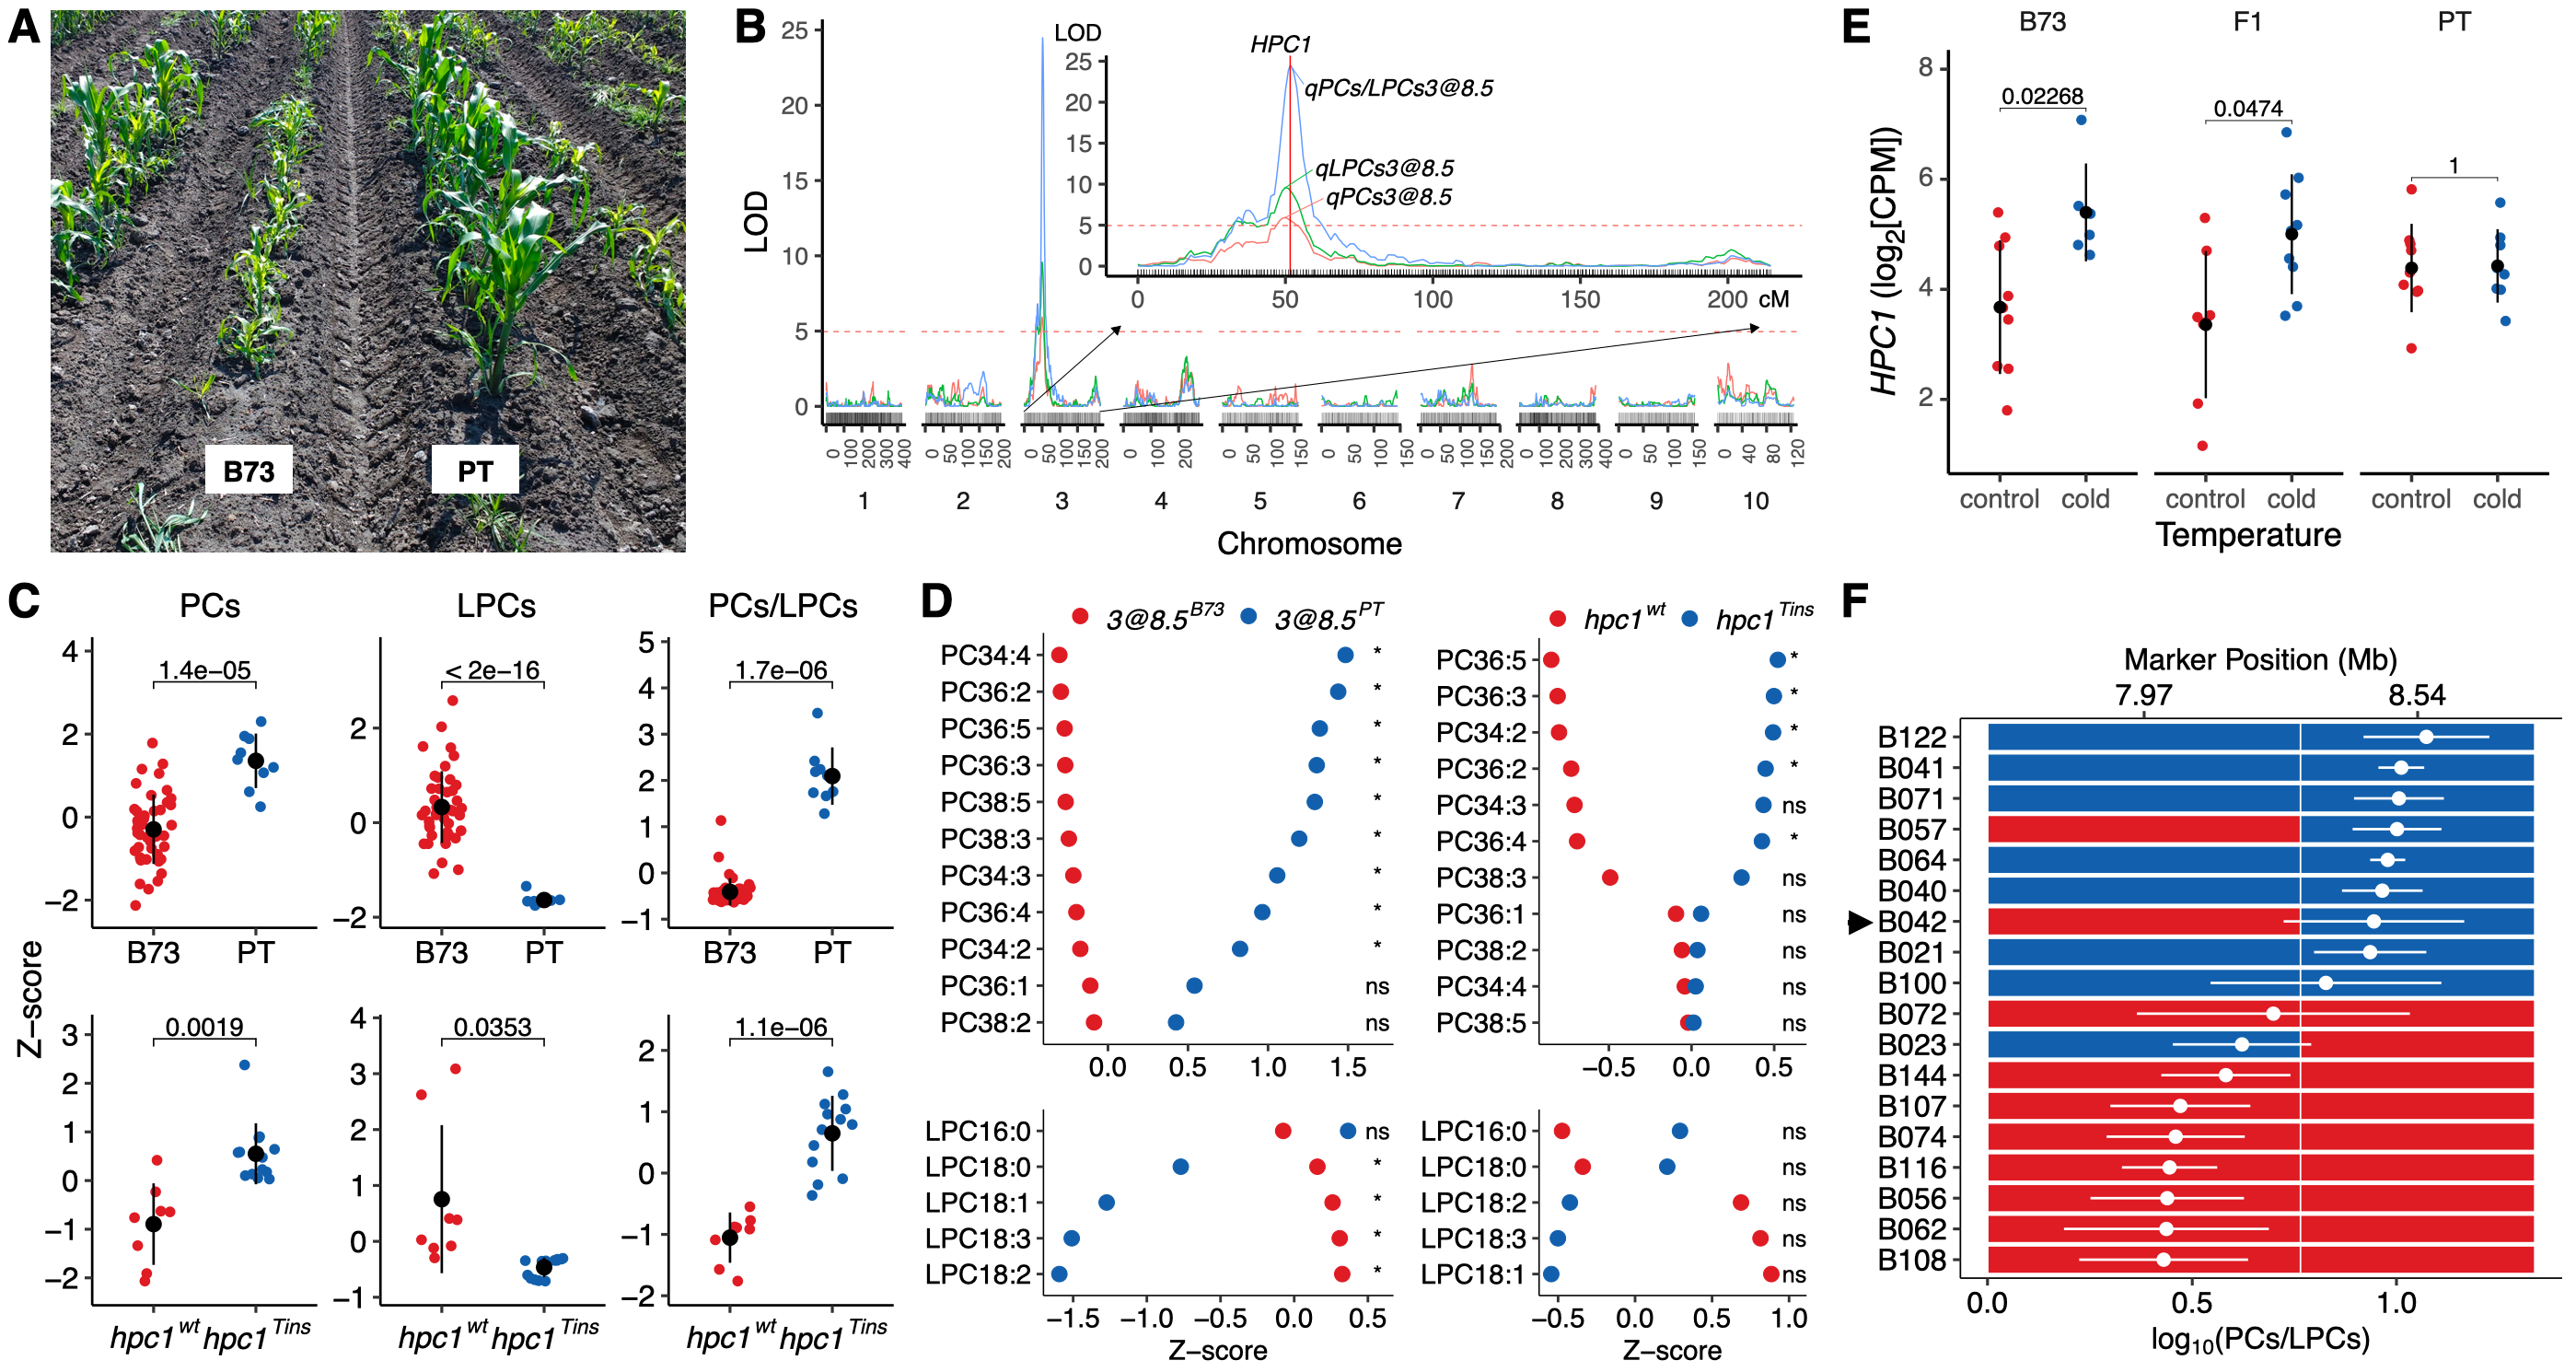
\includegraphics[width=\linewidth]{Chapter-1/figs/Fig_3.png}
\caption[\hpc defines a major QTL explaining PC/LPC conversion]{\textbf{\hpc defines a major QTL explaining PC/LPC conversion.} 
\textbf{(A)} PT and B73 plants growing in the highland Metepec field. 
\textbf{(B)} QTL analysis identified overlapping major QTLs around 8.5 Mb on chromosome 3 for PC and LPC levels and PC/LPC ratio, using data collected from plants grown in highland and lowland fields. 
The QTL peaks coincide with the physical location of \hpc. 
\textbf{(C)} Effect sizes for PCs, LPCs and PC/LPCs (z-score normalized) in RILs that are either homozygous for B73 or PT at 8.5 Mb on chromosome 3 (top row) and CRISPR-Cas9 \textit{hpc1\textsuperscript{Tins}} mutant and wild-type plants (bottom row).
Significant differences were tested by \textit{t}-test; the resulting \textit{p}-values are shown. 
\textbf{(D)} Effect sizes for individual PC and LPC species (z-score normalized) in RILs at 8.5 Mb on chromosome 3 (left) or the CRISPR/Cas9 \textit{hpc1\textsuperscript{Tins}} mutant (right). \textit{*} Significant difference at $p < 0.05$ (\textit{t}-test, after Benjamini \& Hochberg correction), \textit{ns} not significant.
\textbf{(E)} \hpc expression analysis in B73, PT and their F\textsubscript{1} hybrids grown in standard and cold temperatures in a growth chamber. Significant differences were tested by \textit{t}-test with Benjamini \& Hochberg correction; the resulting \textit{p}-values are shown.
\textbf{(F)} PC/LPC ratio for several RILs. RIL B042 (indicated by the black arrow) bears a recombination event 500 bp upstream of the \hpc translation start codon.
In panels (C-F), phenotypes associated with the B73 haplotype are in red; the equivalent values for the PT haplotype are in blue.}
\label{Fig3}
\centering
\end{figure}

Both genes showed strong changes in elevation-dependent allele frequency (\cref{Fig2}D) across Mexican landraces.
\hpc was not an outlier for branch excess between the Andean and the South American lowland accessions.
By contrast, \textit{ZmLPCAT1} was indeed a PBE outlier for all four populations, which may indicate parallel/convergent selection for this gene between Mesoamerican and Andean landraces.
Importantly, both \hpc and \textit{ZmLPCAT1} are annotated as part of pathways with outlier PBE values in all highland populations for ‘phospholipid remodelling’ and ‘PC acyl editing’ (Fig.\cref{Fig1}F, Sup. File 2). 
Taken together, these two independent population genetic approaches show that pathways involved in phospholipid remodelling,  including genes controlling the PC/LPC ratio like \hpc and \textit{ZmLPCAT1}, show strong selection signals in highland maize. 
These results indicate that selection on phospholipid metabolite levels (\cref{Fig1}B-D) is supported at the gene-level by outlier PBE and principal component analysis values \textit{pcadapt} in genes controlling phospholipid biosynthesis and degradation.

%%%%%%%%%%%%%%%%%%%%%%%%%%%%%%%%%%%%%%%%%%%%%%%%%%%%%%%%%%%%%%%%%%%%%%%%%%%%%%%%%%%%
\subsection{A major QTL explaining PC to LPC conversion overlaps \hpc}
%%%%%%%%%%%%%%%%%%%%%%%%%%%%%%%%%%%%%%%%%%%%%%%%%%%%%%%%%%%%%%%%%%%%%%%%%%%%%%%%%%%%
To further characterize the genetic architecture of phospholipid biosynthesis in highland maize, we developed a recombinant inbred line (RIL) BC1S5 population derived from a cross between the temperate inbred line B73 and the Mexican highland landrace Palomero Toluqueño (PT), using B73 as the recurrent parent (75\% B73, 25\% PT) \citep{perez-limon2022}.

The parental PT accession is a popcorn landrace (\textit{palomero} means popcorn in Spanish) from the Toluca Valley in M\'exico (\textit{Mexi5} CIMMYTMA 2233) (\cref{Fig3}A). 
We grew the HiLo diversity panel and the B73 x PT BC1S5 RIL population in the same highland and lowland common gardens and collected samples for glycerolipid analysis.
The locally adapted PT landrace displayed higher fitness than B73 in the highland field (\cref{Fig3}A), probably due to adaptation to low temperatures in this highland environment.  
In the Mexican highlands, values of 5 GDDs per day are typical, while 15-20 GDDs/day are common in lowland environments. 


We detected major quantitative trait loci (QTLs) for the sum of LPC species levels, PC species levels, and the PC/LPC ratio that all mapped to the same locus on chromosome 3, around 8.5 Mb (\cref{Fig3}B). 
We tested for epistatic interactions for LPC levels, PC levels, and the PC/LPC ratio through a combination of R/qtl \code{scantwo} and \code{stepwise} functions \citep{broman2003-ac}.
The three QTLs \textit{qLPCs3@8.5}, \textit{qPCs3@8.5} and \textit{qPCs/LPCs3@8.5} were robust against environmental effects and were detected in both the highland and lowland environments.
The additive effect of the PT allele at these QTLs was associated with high levels of PCs, low levels of LPCs, and consequently high PC/LPC ratios, while the B73 allele had the opposite effect (\cref{Fig3}C, top panel).
Individual PC and LPC species QTLs at this locus \cref{figure:Sup:QTL_effect_sp} showed the same additive effect for the PT allele as the sum of each class (PCs, LPCs, and PCs/LPCs) of species (\cref{Fig3}C, top panel. 
All individual LPC QTLs at the \textit{qLPCs3@8.5} locus corresponded to LPCs that contained at least one double bond in their fatty acid (\cref{figure:Sup:QTL_effect_sp}, Sup. file 3).
\textit{qPCs3@8.5} was driven mainly by PC species with more than two fatty acid double bonds, such as PC 36:5 (\cref{Fig3}D and \cref{figure:Sup:QTL_effect_sp} A-D, Supplementary file 3).
We then sought to identify candidate genes underlying the QTLs on chromosome 3.
The PC/LPC ratio QTL had the highest significance, with a logarithm of the odds (LOD) of 24.5, and explained the most phenotypic variance (87\%). 
The underlying QTL interval contained 72 genes within its 1.5 LOD drop confidence interval (7.9-10 Mb). 
We hypothesized that the metabolic phenotypes we observed might be due to a gene involved in PC-LPC conversion.  
The maize genome encodes 75 putative phospholipases (\cref{figure::Sup:HPC1_misc}A), of which half are predicted to be phospholipase A1-type (PLA1) (\cref{figure::Sup:HPC1_misc}B).  
Notably, \hpc mapped within the interval (position on chromosome 3: 8,542,107 bp to 8,544,078 bp), making it a high confidence candidate causal gene (\cref{Fig3}B). 
HPC1 was predicted to have phospholipase A1-Igamma1 activity and can be classified as a PC-hydrolyzing PLA1 Class I phospholipase based on its two closest Arabidopsis orthologs (encoded by \textit{At1g06800} and \textit{At2g30550}) \citep{ryu2004-iv}. 
PLA1-type phospholipases hydrolyze phospholipids in the \textit{sn-1} position and produce a lyso-phospholipid and a free fatty acid (\cref{figure::Sup:HPC1_misc}B). 
In B73, \hpc was one of the most highly expressed phospholipase genes, with expression almost exclusively restricted to vegetative leaves (V4-V9) (\cref{figure:Sup:B73_expression}A) \citep{stelpflug2016-vr}, which was the biological material we sampled for glycerolipid analysis. 
In B73 leaves, \hpc was also the most highly expressed gene within the QTL interval (\cref{figure::Sup:HPC1_misc}C) \citep{stelpflug2016-vr}.
Class I phospholipases are chloroplast-localized proteins; in agreement, we identified a chloroplast transit peptide (CTP) at the beginning of the predicted HPC1 sequence using the online tool ChloroP \citep{emanuelsson1999-rs}.
We validated the chloroplast localization of HPC1 by transiently expressing a construct encoding the HPC1 CTP fragment fused to green fluorescent protein (GFP) in \textit{Nicotiana benthamiana} leaves (\cref{figure:Sup:HPC1_organelle}).

The effect of \hpc on PC/LPC levels may be caused by misregulation of \hpc expression in highland landraces and/or by a mutation affecting HPC1 enzymatic activity. 
To distinguish between these two possibilities, we analyzed \hpc expression in B73, PT, and the corresponding F\textsubscript{1} hybrid plants grown at high and low temperatures to simulate highland and lowland conditions, respectively (\cref{Fig3}E). 
Under cold conditions, \textit{HPC1-B73} was up-regulated, but \textit{HPC1-PT} was not (\cref{Fig3}E). 
The lack of up-regulation in cold conditions of \hpc may explain the high PC/LPC levels in PT.
However, \hpc expressed to the same levels in B73 and PT under control conditions.
In the F\textsubscript{1} hybrids, \hpc expression was consistent with a dominant B73 effect.
We also observed a dominant B73 effect at the metabolic level when we analyzed B73 x PT RILs that are heterozygous at the \hpc locus
(\cref{figure::Sup:HPC1_misc}D).
Variation in \hpc may also affect enzymatic activity of the HPC1-PT variant. 
To test this hypothesis we sequenced three B73 x PT RILs (B021, B042, B122) that are homozygous for the \textit{HPC1-PT} allele.
We discovered a recombination point between 493 and 136 bp upstream of the \hpc translation start codon (\cref{Fig3}F, \cref{figure:Sup:hpc1_promoter}) in RIL B042, resulting in a chimeric locus with the coding region from PT combined with a promoter segment from B73.
PC/LPC levels in RIL B042 were similar to other RILs that are homozygous for the PT haplotype at the 8.54 Mb marker at the QTL peak (\cref{Fig3}F). 
This result supports the hypothesis that the metabolic effect in the B73 x PT RILs is likely due to an impaired function of the HPC1-PT enzyme rather than to changes in the \textit{HPC1-PT} regulatory region.
However, regulatory variants in the first 500 bp of the promoter may also impact expression levels in RILB042.

If \hpc is the underlying causal gene of this QTL, the observed metabolic phenotypes would be consistent with a reduction or loss of HPC1-PT enzyme function, leading to higher levels of PCs and lower levels of LPCs in the PT background. 
To test this hypothesis we generated mutants in \hpc via clustered regularly interspaced short palindromic repeats (CRISPR)/CRISPR-associated nuclease (Cas9)-mediated genome editing (\cref{figure:Sup:CRISPR_effect}A) in the B104 inbred, a temperate stiff stalk inbred derived from the Iowa Stiff Stalk Synthetic population like B73. 
We identified two transgenic mutants, hereafter designated \textit{hpc1\textsuperscript{CR T ins}} and \textit{hpc1\textsuperscript{CR T del}} (\cref{figure:Sup:CRISPR_effect}A).
We then measured PC and LPC species in wild-type and mutant plants grown under long day conditions.  
The phospholipid profiles of the \textit{hpc1\textsuperscript{CR}} plants 
replicated those of the \textit{PT} allele in the RILs (\cref{Fig3} C-D bottom panels and \cref{figure:Sup:CRISPR_effect}B), confirming that the \textit{HPC1-PT} allele impairs HPC1 function and thus underlies the QTL on chromosome 3 around 8.5 Mb. 
Lastly, we \textit{in vitro} translated HPC1-B73 and HPC1-PT  versions of the protein in a cell-free system and incubated them with various phospholipid substrates. 
We then measured the amount of phospholipid substrate and lyso-phospholipid product for each compound (\cref{figure:Sup:MS_spectra}). 
This experiment confirmed that both HPC1 variants have PLA1 activity and suggested that HPC1-B73 may have higher activity on substrates like PC36:4 that show stark differences in abundance between highland and lowland lines, as well as in \textit{hpc1\textsuperscript{CR}} lines.
Together, the RIL and CRISPR mutant results showed that \hpc underlies a major metabolic QTL explaining PC/LPC ratio. 
A mutation in the flap-lid domain of HPC1 affecting substrate accessibility likely leads to impaired function in the highland PT allele.

%%%%%%%%%%%%%%%%%%%%%%%%%%%%%%%%%%%%%%%%%%%%%%%%%%%%%%%%%%%%%%%%%%%%%%%%%%%%%%%%%%%%%%%%%%%%%%%%%%%%%%%% 
\subsection{\hpc shows strong elevation-dependent antagonistic pleiotropy in Mexican landrace fitness phenotypes}
%%%%%%%%%%%%%%%%%%%%%%%%%%%%%%%%%%%%%%%%%%%%%%%%%%%%%%%%%%%%%%%%%%%%%%%%%%%%%%%%%%%%%%%%%%%%%%%%%%%%%%$$
Our selection and QTL analysis provided strong evidence that \hpc is under selection in highland maize and controls phospholipid metabolism. 
To evaluate the possible fitness effects of HPC1 variation in locally adapted landraces across M\'exico, we re-analyzed phenotypic data from a previously reported F1 association mapping panel \citep{romero_navarro2017-cn, gates2019-xu} composed of about 2,000 landrace F1s grown in 23 common garden environments across an elevation gradient.  
We then fitted a model to estimate the effect of variation at \textit{HPC1-PT} on the relationship between fitness traits and elevation \citep{runcie2019-Gr}.
\hpc was a clear outlier in a genome wide association study (GWAS) of genotype-by-elevation fitness traits like flowering time and yield (\cref{figure:Sup:GxE_scan}A-B), indicating that elevation-dependent variation at \hpc not only has an effect on phospholipid levels but also on fitness traits.
Indeed, variation at \hpc showed significant genotype $\times$ elevation effects for several fitness traits (\cref{Fig5}A). 
The effect of \hpc on flowering time revealed antagonistic pleiotropy between highland and lowland environments (\cref{Fig5}A). 
The highland \textit{HPC1-PT} allele was associated in low elevations with delayed flowering, increasing days to anthesis (DTA) by about one day.
Meanwhile the same allele exhibited accelerated flowering at high elevation (with a decrease in DTA of almost one day, \cref{Fig5}A).
Variation at \hpc also displayed conditional neutrality on fresh ear weight and grain weight per hectare traits: the highland allele had no effect in lowland environments but was associated with greater values in highland environments (\cref{Fig5}A).
We also checked previous reports for associations between \hpc and flowering time in other populations through the MaizeGDB \citep{woodhouse2021-wd} genome browser. 
We in fact found a significant flowering time SNP in the \hpc coding sequence (\cref{Fig5}B) for the Nested Association Mapping (NAM) population \citep{wallace2014-yy}. 
This additive flowering time locus is only 6 bp from the focal SNP we used to test  $G \times E$ at \hpc in the SEEDs panel (\cref{Fig4}). 
Variation at this SNP correlated with a reduction in flowering time of 8.5 hours, relative to B73, and explained 1.12\% of the trait variance, which is about one third of the largest effect observed for flowering time variation in the NAM population. 

\begin{figure}[htp]
\centering
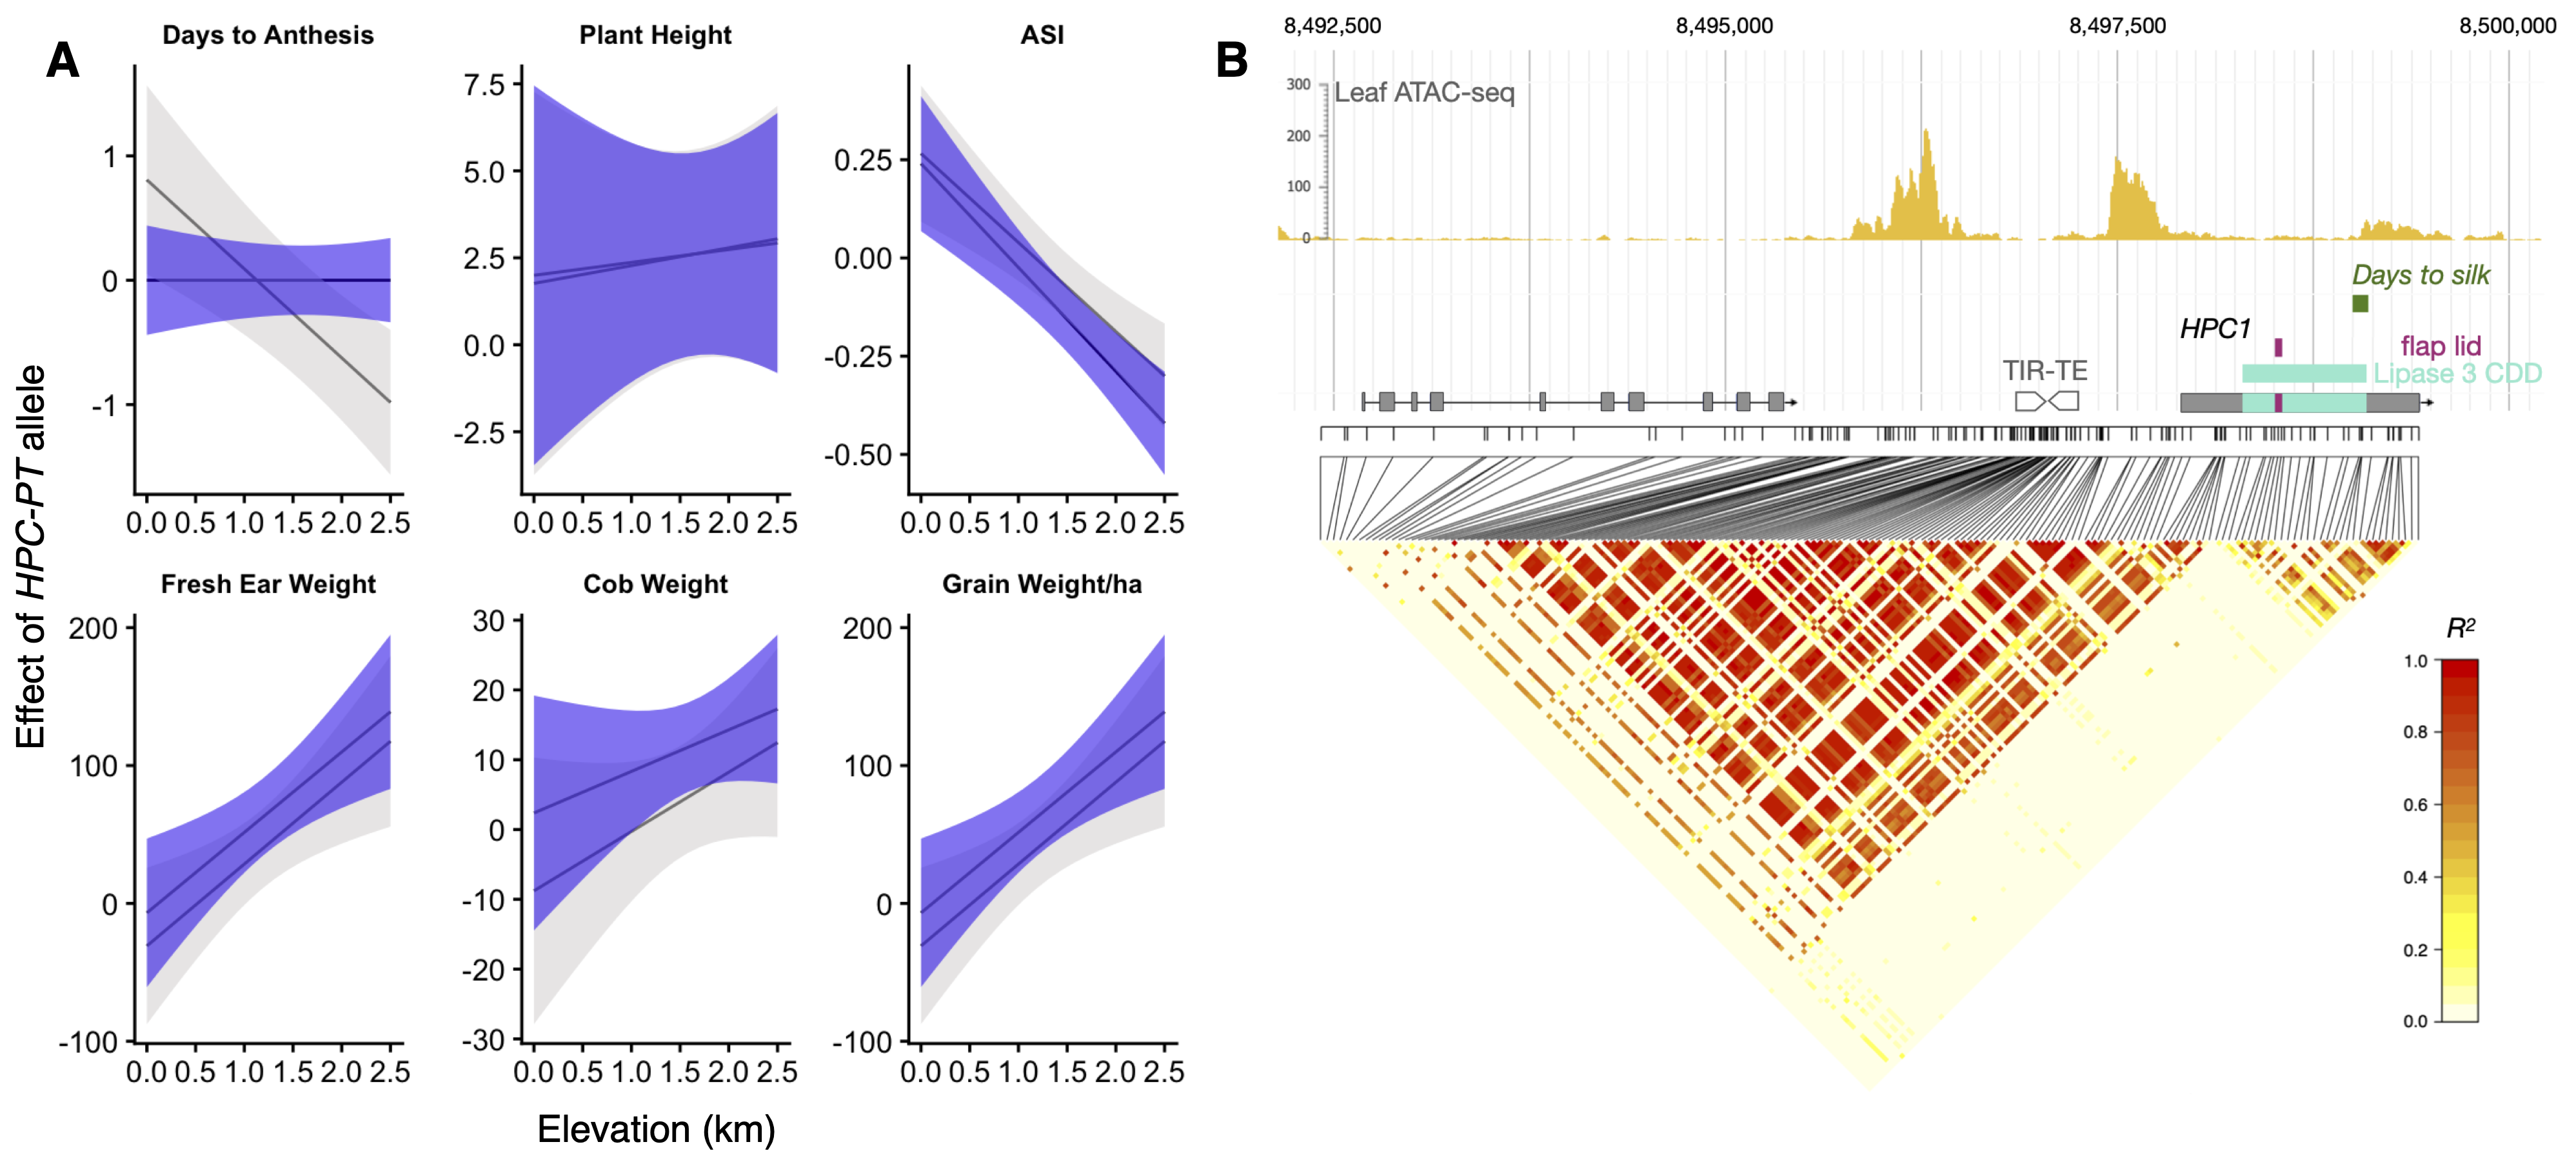
\includegraphics[width=\linewidth]{Chapter-1/figs/Fig_5.png}
\caption[Fitness effects of the \textit{HPC1-PT} allele and \hpc LD analysis.]{\textbf{Fitness effects of the \textit{HPC1-PT} allele and \hpc LD analysis.} \textbf{(A)}
We used best linear unbiased predictions (BLUPs) and GBS data from 2,700 landrace topcrossess from \citep{gates2019-xu}, evaluated in 23 common gardens at different elevations in M\'exico. 
We modeled each trait as a function of the \textit{HPC1-PT} genotype, trial elevation, and tester line, with controls for main effects and responses to elevation of the genomic background. 
Gray lines and ribbons show estimates of the effect of the highland allele of \textit{HPC1-PT} as a function of common garden elevation ± 2 standard errors of the mean, using the \textit{GridLMM} package \citep{runcie2019-Gr}. 
Purple lines show estimates of the \textit{HPC1-PT} effect in a model that also adjusts for effects of days to anthesis. ASI, anthesis to silking interval. 
\textbf{(B)} Linkage disequilibrium and genomic features of \hpc and upstream region. 
LD heatmap drawn with \citep{zhou2019} from HapMap 3 data. 
Top track shows leaf ATAC-seq peaks in B73, data from \citep{ricci2019-zj}.
The regions coding for the lipase and flap-lid domains are highlighted on the \texit{HPC1} gene model. 
See \ref{Fig4}A for further details.
Days to Anthesis indicates the GWAS SNP on the lipase domain from \citep{wallace2014-yy}.
TIR-TE, terminal inverted repeat transposable element.
Tracks obtained from MaizeGDB B73 V5 browser \citep{woodhouse2021-wd}.}
\label{Fig5}
\end{figure}

We then used genetic marker data from the HapMap 3, which includes the NAM parents, \citep{bukowski2017-ng} to analyze linkage disequilibrium (LD) of the \hpc region (\cref{Fig4}B).
We detected a strong LD block of about 150 bp in length in the coding sequence that includes the focal SNP mentioned above (\cref{Fig5}A,B). 
We identified another LD block covering the 5' region of \hpc and the promoter region up to 2 kb upstream of \hpc (\cref{Fig5}B). 
Interestingly, this second LD block on the promoter overlapped with two strong ATAC-seq (assay for transposase-accessible chromatin followed by sequencing) peaks identified in B73 (\citep{Ricci2019-zj}, \cref{Fig5}B).
These results confirmed that the SNPs associated with fitness traits like flowering time on the \hpc coding sequence are not linked to other SNPs upstream of the \hpc coding sequence.
However, the SEEDs data set lacks GBS markers for several kb upstream of \hpc, raising the possibility of a second regulatory variant in the promoter (\cref{Fig4}B) that might have an effect on \hpc expression. 
We further evaluated the possible effect of \hpc on flowering using both \textit{hpc1\textsuperscript{CR}} mutants in long-day conditions during the Summer of 2021 in Raleigh, NC. 
Although the mutants showed high PC/LPC ratios, we observed no significant difference in flowering time relative to the wild type (\cref{figure:Sup:CRISPR_effect}C). 
As shown in (\cref{Fig4}A) the effect of the \hpc allele on flowering time has a strong G x E pattern and we only observe a significant effect in very high or low elevations. 
We speculate that the absence of significant differences in the B104 CRISPR mutants in Raleigh conditions could partly be explained by the strong G X E effect of \hpc and/or genetic background effects. 

In summary, the SNPs in the short, lipase-domain-encoding LD block of \hpc show strong genotype x elevation fitness effects in both Mexican landraces grown across multiple altitudes and the NAM population.
The phospholipid changes induced by \hpc have physiological effects that may explain the strong selection of \hpc in highland environments.
%%%%%%%%%%%%%%%%%%%%%%%%%%%%%%%%%%%%%%%%%%%%%%%%%%%%%%%%%%%%%%%%%%%%%%%
\subsection{\textit{HPC1-PT} was introgressed from teosinte \mex and is conserved in Flint inbred lines}
%%%%%%%%%%%%%%%%%%%%%%%%%%%%%%%%%%%%%%%%%%%%%%%%%%%%%%%%%%%%%%%%%%%%%%
We explored the segregation of the V211I SNP among other highland maize varieties.
We detected the PT allele at high frequencies in highland landraces from M\'exico and Guatemala. 
In addition, the PT allele segregated in Southwestern US landraces. 
The B73 allele was fixed in lowland Mexican, South American, and Andean landraces (\cref{Fig6}A). 
These results were consistent with our PBE results (\cref{Fig2}F).
The PT allele was also present in one fourth of all teosinte \parv accessions tested and in both \mex accessions reported in Hapmap 3 \citep{bukowski2017-ng} (\cref{Fig6}A). 
This observation prompted us to examine whether the PT allele was the result of post-domestication introgression from teosinte \mex during maize highland colonization, or whether it was selected from \parv standing variation.
To test for introgression from \mex, we used \(f_d\) data from \citep{gonzalez-segovia2019-jy} and established that the genomic region containing \hpc shows signatures of introgression from \mex into highland maize (\cref{Fig6}B).
We then performed a haplotype network analysis using SNP data from the \hpc coding region of 1,160 Mexican accessions from the SeeD Dataset \citep{romero_navarro2017-cn} that are homozygous for all SNPS across the coding region and the teosinte inbred lines (TILs) from Hapmap 3 \citep{bukowski2017-ng}.   
We identified nine haplotype groups that cluster mainly based on elevation (\cref{Fig6}C). 
The two major groups, II and VI, contained mainly lowland and highland landraces, respectively. 
The two \mex teosinte inbred lines (TIL08 and 25) belonged to group IV  (\cref{Fig6}C) together with highland landraces primarily collected in the Trans-Mexican Volcanic Belt (30/36 from the highlands of Jalisco, Michoacán, M\'exico, Puebla, and Veracruz).
We then examined whether this \mex haplotype (denoted \textit{ZxHPC1}) that is introgressed into Mesoamerican highland maize was also present in modern maize inbred lines. 

To this end, we performed a neighbor-joining cluster analysis using Hapmap 3 \citep{bukowski2017-ng} inbred lines including those from the 282 inbred panel, Teosinte inbred lines, German lines, and PT. 
We identified two main groups, one containing the \textit{HPC1-PT} haplotype and the other containing the \textit{HPC1-B73} haplotype.
PT and the teosinte \mex inbred lines TIL08 and TIL25 clustered together with Northern European Flint inbred lines such as EP1, UH008, and UH009 (\cref{Fig6}D). 
Other Northern US flints, e.g., CM7, were also closely related to the \mex \textit{ZxHPC1} haplotype. 
These data suggest that after introgression into highland maize, the \textit{ZxHPC1} haplotype was maintained in Flint materials adapted to cold environments in the Northern US, Canada, and Europe. 
We then used a large gene expression dataset consisting of multiple developmental stages of the 282-maize diversity panel \citep{kremling2018-gn} and phenotypic datasets collected from the same panel grown in long days and short days.
Notably, \hpc expression levels were highly correlated with flowering time in both long and short days. 
Lines carrying the \textit{HPC1-PT} allele were characterized by lower \hpc expression and earlier flowering times relative to lines carrying the \textit{HPC1-B73} allele (\cref{Fig6}E).
Taken together, these data show that \hpc was introgressed from teosinte \mex into highland maize and that this introgression was carried over into high latitude-adapted modern inbred lines with low \hpc expression and early flowering.
\begin{figure}[!ht]
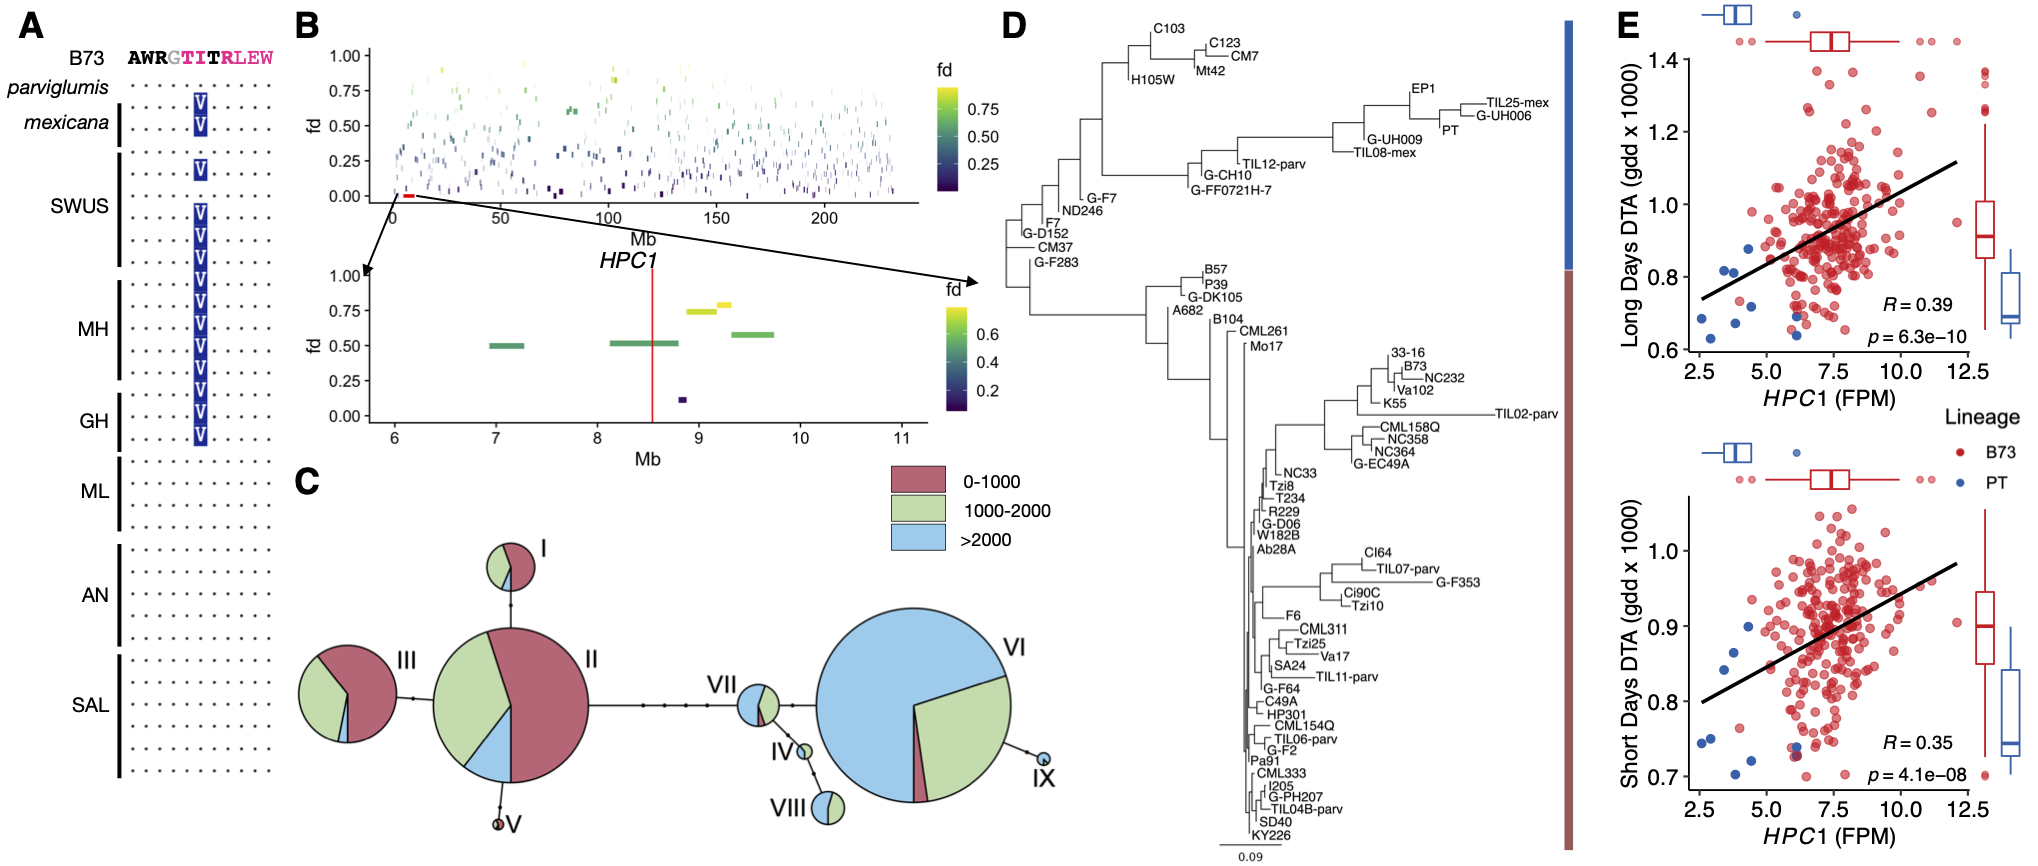
\includegraphics[width=\linewidth]{Chapter-1/figs/Fig_6.png}
\caption[Introgression of teosinte \mex into maize \hpc.]{\textbf{Introgression of teosinte \mex into maize \hpc.}  
\textbf{A)} Alignments around the V211I polymorphism in the flap-lid domain of HPC1 in B73, \mex and \parv and landraces of the Southwestern US (SWUS), Mexican Highland (MH) and Lowlands (ML), Guatemalan Highlands (GH), Andes (AN) and South America Lowlands (SAL).
\textbf{B)} \(f_d\) analysis of the \mex introgression. Data were obtained from \citep{Gonzalez-Segovia2019-jy}. 
\textbf{C)} Haplotype network analysis of SNPs within the \hpc coding region, using 1,060 Mexican homozygous individuals from the SeeD dataset. Haplotypes are color-coded by elevation: red: 0-1000 masl, green: 1000-2000 masl, blue >2000 masl.
\textbf{D)} Cluster analysis of the \hpc coding region using a sample of Hapmap3 inbred lines and the PT landrace.
\textbf{E)} Correlation between \textit{HPC1-PT} expression and days to anthesis (DTA) in plants grown in short or long days. 
Inbred lines from the PT lineage shown in panel C are indicated in blue and inbred lines from the B73 lineage are in red;
data from \citep{kremling2018-gn}.}
\label{Fig6}
\end{figure}

\section{Discussion}

Understanding the genetic, molecular, and  physiological basis of crop adaptation to different environments and the role that wild relatives have played in these processes is relevant for the identification of favorable genetic variation that can be used to improve modern crops.
The repeated events of maize adaptation to highland environments constitute an excellent natural experiment to study local adaptation. 
Recent studies \citep{wang2020-mp, takuno2015-uj, crow2020-gene} have helped expand our understanding of the genetic basis underlying maize highland adaptation. 
However, the responsible molecular, physiological, and genetic mechanisms underlying maize highland adaptation and the possible role of highland maize traits in modern, commercial varieties remain largely unknown.
Phospholipids are key structural components of plant membranes that also function as signaling molecules during adaptation to stresses that would be prevalent in highland environments \citep{ryu2004-iv, nakamura2017-vb} such as low phosphorus availability \citep{veneklaas2012-ls, cruz-ramirez2004-ib, lambers2012-an} and low temperatures \citep{degenkolbe2012-wf, welti2002-uk, marla2017-ph}. 
In Arabidopsis and rice (\textit{Oryza sativa}, phospholipid species regulate flowering time via interactions with \textit{Arabidopsis} FT and rice Heading date 3a (Hd3a), respectively \citep{nakamura2014-qf, susila2021-dz, qu2021-wc}. 
Flowering time is a major driver of maize adaptation to highland environments \citep{romero_navarro2017-cn, gates2019-xu, mercer2019-vj} and to northern latitudes \citep{hung2012-ms, swarts2017-ge}.

Genes involved in the biosynthesis and degradation of phospholipids appeared to have been repeatedly selected in several highland maize populations of North America, Central America, and South America (Figures \cref{Fig1} and \cref{Fig2}). 
\textit{ZmLPCAT1} and \hpc were two such genes with the strongest, repeated signals of selection, as measured by PBE and \textit{pcadapt} in highland populations (\cref{Fig2}). 
In a previous study, \textit{ZmLPCAT1} exhibited high $F_{ST}$ values when highland and lowland landraces were compared \citep{takuno2015-uj}.
In temperate inbred lines, \hpc was up-regulated while \textit{ZmLPCAT1} was down-regulated by cold stress (\cref{figure:Sup:B73_expression}B-C) \citep{waters2017-nat}.
These expression patterns are in agreement with the high and low PC/LPC ratios observed in our experiments. 
Furthermore, we determined here that \hpc is up-regulated in B73 and B73 x PT F\textsubscript{1} hybrids after cold exposure. 
By contrast, the \textit{HPC1-PT} and \textit{HPC1-B73} alleles were expressed to comparable levels in control conditions, and the \textit{HPC1-PT} allele was not induced upon cold conditions (\cref{Fig3}E).
Selection at these two loci is likely to have driven the high PC/LPC ratio we observed in highland Mexican landraces (\cref{Fig1}). 

Our QTL analysis of the PC/LPC ratios in a B73 x PT mapping population and in the \textit{hpc1\textsuperscript{CR}} mutant alleles demonstrates that the highland \textit{HPC1-PT} allele results in an enzyme with impaired function that alters highland Mexican maize PC metabolism, leading to higher PC/LPC ratios (\cref{Fig3}, \cref{figure:Sup:CRISPR_effect}B). 
Adaptive loss-of-function mutations can be an effective way to gain new metabolic functions in new environmental conditions \citep{hottes2013-np}.
Taking advantage of the conserved lipase domain of HPC1 in bacteria, we used a new method that can identify how genetic variation in DNA regions encoding protein domains is correlated with optimal growth temperature of bacteria \citep{jensen2021-iv, jensen2021-zm}.
The probable causal SNP in HPC1 changed an amino acid in the flap-lid domain of HPC1 (\cref{Fig5}A) that may affect substrate  accessibility and/or substrate binding (\cref{Fig5}A). 
Indeed, the flap-lid domain has been the target of biotechnological modification for lipases \citep{khan2017-ua}.
The region encoding the flap-lid domain was located at a recombination point that separates two clear LD blocks. 
The first LD block covered a 2-kb promoter region of \hpc and the first 600 bp of \hpc, while the second covered the rest of the \hpc coding sequence. 
In fact, this pattern is characteristic of selective sweeps that leave two LD blocks on either side of the adaptive mutation sweep \citep{kim2004-pa}. 
LD analysis together with the open chromatin detected by ATAC-seq that overlaps the same promoter region (\cref{Fig4}B) and the correlation between \hpc expression and flowering time (\cref{Fig6}E) presented here suggest a possible transcriptional regulation of \hpc that may act additively with the coding sequence variation we described. 

Why were the metabolic changes induced by HPC1 variation selected for in highland maize?
PC metabolism is intimately connected to multiple stress responses and developmental pathways; alterations in PC amounts and PC/LPC ratios affect overall plant fitness.
The \textit{qPC/LPC3@8.5} QTL is driven by individual QTLs for PC and LPC species with high levels of unsaturated fatty acids (\cref{Fig3}D).
Several of these species, like PC 36:5 and LPC 18:1 (\cref{Fig3}D, Sup. File 3), have been shown to display similar patterns during Arabidopsis cold acclimation \citep{Welti2002-uk} and sorghum (\textit{Sorghum bicolor}) low temperature responses \citep{marla2017-ph}.
PC 36:5 also showed high $Q_{ST}$ values when comparing highland and lowland landraces from both Mesoamerica and South America (\cref{fig1}C-D, Sup. File 5).
In maize, \hpc expression is under the control of the circadian clock \citep{khan2010-iv} with a peak at the end of the day. 
In Arabidopsis, highly unsaturated PC (34:3, 34:4, 36:5, 36:6) species increase in the dark \citep{maatta2012-ip}. 
This peak in contents coincides in maize with low \hpc expression levels during the same dark hours \citep{khan2010-iv}.
PC, and lipid metabolism in general, is also intimately connected to flowering time. 
For instance, PCs were shown to bind to Arabidopsis FT in the shoot apical meristem to hasten flowering \citep{nakamura2014-qf, nakamura2019-ht} by unknown cellular mechanisms. 
Similarly, PG species can sequester FT in phloem companion cells in low temperatures \citep{susila2021-dz} and then release FT into the phloem later after temperatures increase, allowing FT reach the shoot apical meristem.   
In agreement with an effect of lipids on flowering time, overexpression of a gene encoding a secretory phospholipase D delayed heading time in rice \citep{qu2021-wc}.
In line with a role for phospholipids in flowering, we established that genetic variation at SNPs within the region of \hpc encoding the lipase domain exhibits a strong interaction with elevation for the highland \textit{HPC1-PT} allele. 
This variation leads to a delay in flowering time in low elevations and an acceleration at high elevations, both of which close to one day in amplitude. 
Interestingly, the effect of the highland \hpc allele exhibited typical conditional neutrality in yield-related traits, with higher fitness conferred by the \textit{HPC1-PT} allele in highlands (\cref{Fig4}A). 
In the NAM population, we identified another SNP mapping to the region encoding the lipase domain that is associated with a hastening of flowering time by eight hours with respect to B73 \citep{wallace2014-yy}, further supporting the role of \hpc in controlling flowering time. 
Analysis of \hpc CRISPR mutant alleles in the B104 background grown in Raleigh displayed a PC/LPC phenotype that mimicked the highland allele (\cref{figure:Sup:CRISPR_effect}A-B) but not a flowering time phenotype, probably due to the strong G x E effect of \hpc and/or genetic background effects. 

The strong G x E effect we observed in \hpc is similar to the well-known teosinte \mex introgression \textit{inv4m} \citep{crow2020}. 
In fact, our analysis showed that \hpc is indeed another introgression from teosinte \texit{mexicana} (\ref{Fig6}A-C). 
Recent analysis using sympatric teosinte and maize populations across elevation gradients in Mexico further supports the introgression of \mex at \hpc and shows that the \mex ancestry of \hpc increases at a rate of +0.079 per 100 m of elevation \citep{calfee2021-mr}.
We further demonstrated that the \texit{mexicana} intogression at \hpc is conserved in high latitude-adapted Flint lines from both Europe and the USA (\cref{Fig6}D).
\textit{HPC1} in inbred lines carrying the highland \textit{ZxHPC1} \mex haplotype was expressed at low levels and resulted in earlier flowering (\cref{Fig6}E) \citep{kremling2018-gn}.  

Adaptation to higher latitudes involved a reduction of photoperiod sensitivity and flowering time that enabled maize to thrive in longer day conditions characteristic of the growing season at high latitudes \citep{hung2012-ms, Swarts2017-ge, yang2013-lg, huang2018-ga}.
Additive mutations in the regulatory region of the gene \textit{ZCN8} \citep{lazakis2011-nq}, including a teosinte \mex introgression, lead to higher expression of \textit{ZCN8}, which contributes to maize adaptation to long days in temperate conditions \citep{guo2019-pn}.
\textit{ZCN8} is a close ortholog of Arabidopsis \textit{FT}, whose encoding protein interacts with several species of phospholipids to modulate flowering time \citep{nakamura2014-qf, susila2021-dz}. 
A similar interaction was also demonstrated for the rice FT ortholog Hd3a, \citep{qu2021-wc} and we hypothesize that the same may be occurring in maize. 
Comparison of docking simulations of phospholipids with ZCN8 using the Arabidopsis FT crystal structures as a model \citep{nakamura2019-ht} showed similar PC interactions in ZCN8 (\cref{figure:Sup:Docking}).
We corroborated this interaction via mass spectrometry analysis of lipids bound to ZCN8 heterologously produced in yeast (\cref{figure:Sup:ZCN8-PC}). 

In summary, we used a combination of genomic scans, linkage mapping, lipidomics and reverse genetics to identify and clone the adaptive gene \hpc, introgressed from teosinte  \mex, in highland maize landraces. 
HPC1 variants lead to a major reorganization of phosphatidylcholine metabolism. 
We showed that the fitness advantage conferred by the \hpc highland \mex allele is due, at least in part, to its association with flowering time. 
This effect may have contributed to adaptation of maize to colder, higher latitudes.

Our work is the first to identify the important role of a gene controlling phospholipid metabolism in plant local adaptation and further supports the emerging role of phospholipid metabolism in fine-tuning flowering time across different plant species \citep{nakamura2014-qf, susila2021-dz, guo2019-pn}.
This study highlights the largely underappreciated role of highland maize and highland teosinte \mex in modern maize.

\printbibliography[heading=subbibintoc, title=References]
